\chapter{Discussion}

In this chapter, we review results of our experiments and discuss applications of the analyzed models in other systems. We also give tips on how to perhaps further improve performance of our models and which aspects of human memory could be considered in future research.

\section{Results}

In chapter~\ref{analysis}, we analyzed several models based on timing information (taking into account either ages of past trials of items or past response times of students). Most promising results in the context of learning geography facts shows the PFA/E/T model with a staircase time effect function, although the power function proves to be almost as equally a good choice. Main advantage of the staircase function is that the parameters are easy to learn for the purpose of online learning, i.e. there is no need to periodically run parameter optimization procedure since the parameters are slightly adjusted with each new answer.

The PFA/G/T model suffers from the inability to account for multiple-choice questions. It might be interesting to analyze the models on data from adaptive systems where questions with multiple-choice options are not used---this is not possible using the data set described in section~\ref{data-set} since the system adaptively selects number of options in multiple choice tests, i.e. filtering out all multiple-choice questions creates data set with skewed difficulties and abilities of students.

The PFA/E/RT model that considers past response times of students shows in most cases only a very small improvement. However, very interesting results provides the PFA/G model with values of the decay factor lower then 0.5, this may indicate that the past trials of items do not actually influence model's performance in the context of learning geography facts as much as we thought. When we compare the PFA/G model and the PFA/G/T model, it seems that penalizing old trials based on order of answers leads in most cases to a better performance than the penalty of trials based on timing information.

\section{Applications and Recommendations}

Currently, models used in the adaptive system Outline Maps do not take into account ages of past trials. We have demonstrated that the timing information improves model's performance and thus, the extensions of presented models should be considered in production. As we already discussed in previous section, the best choice is the PFA/E/T model with a time effect function fitted by gradient descent described in chapter~\ref{approx-gradient}.

Another application of our models could be considered in the adaptive system for practicing medical anatomy (\url{practiceanatomy.com}) targeted mostly at medical students. The system allows the practice of various organ systems, body parts, bones, muscles, etc. The evaluation of our models on data from students who practice anatomy could also open interesting questions about difficulty of items and the effect of forgetting where most students are collage students.

\section{Possible Extensions and Alternative Models}

The examined models approximate the effect of human memory decay with a time effect function which ignores some very important aspects of memory and forgetting. For example, in our models the spacing effect is completely disregarded. One extension of the PFA/G/T model could reuse some properties of the memory activation equation~\ref{eq-pavlik-activation} described in chapter~\ref{spacing-effect}. Next, an extension of the PFA/G/T model which considers multiple-choice questions might also be possible and could significantly improve its performance.

Another extension of the models could consider the fact that students mix up the places that are, for instance, geographically very close, have similar names, or seem somehow similar for entirely different reasons. Students typically know the approximate geographical location of the Nordic countries, however, they might struggle when determining exact location of each country, often they confuse Norway with Sweden as can be seen in Figure~\ref{fig:confusion-network}. If a students chooses Finland when the highlighted place is actually Norway, it usually does not mean that they have no knowledge of the country's location. In such cases it might be more accurate to slightly increase student's memory activation of the place.

\begin{figure}[htbp]
  \centering
  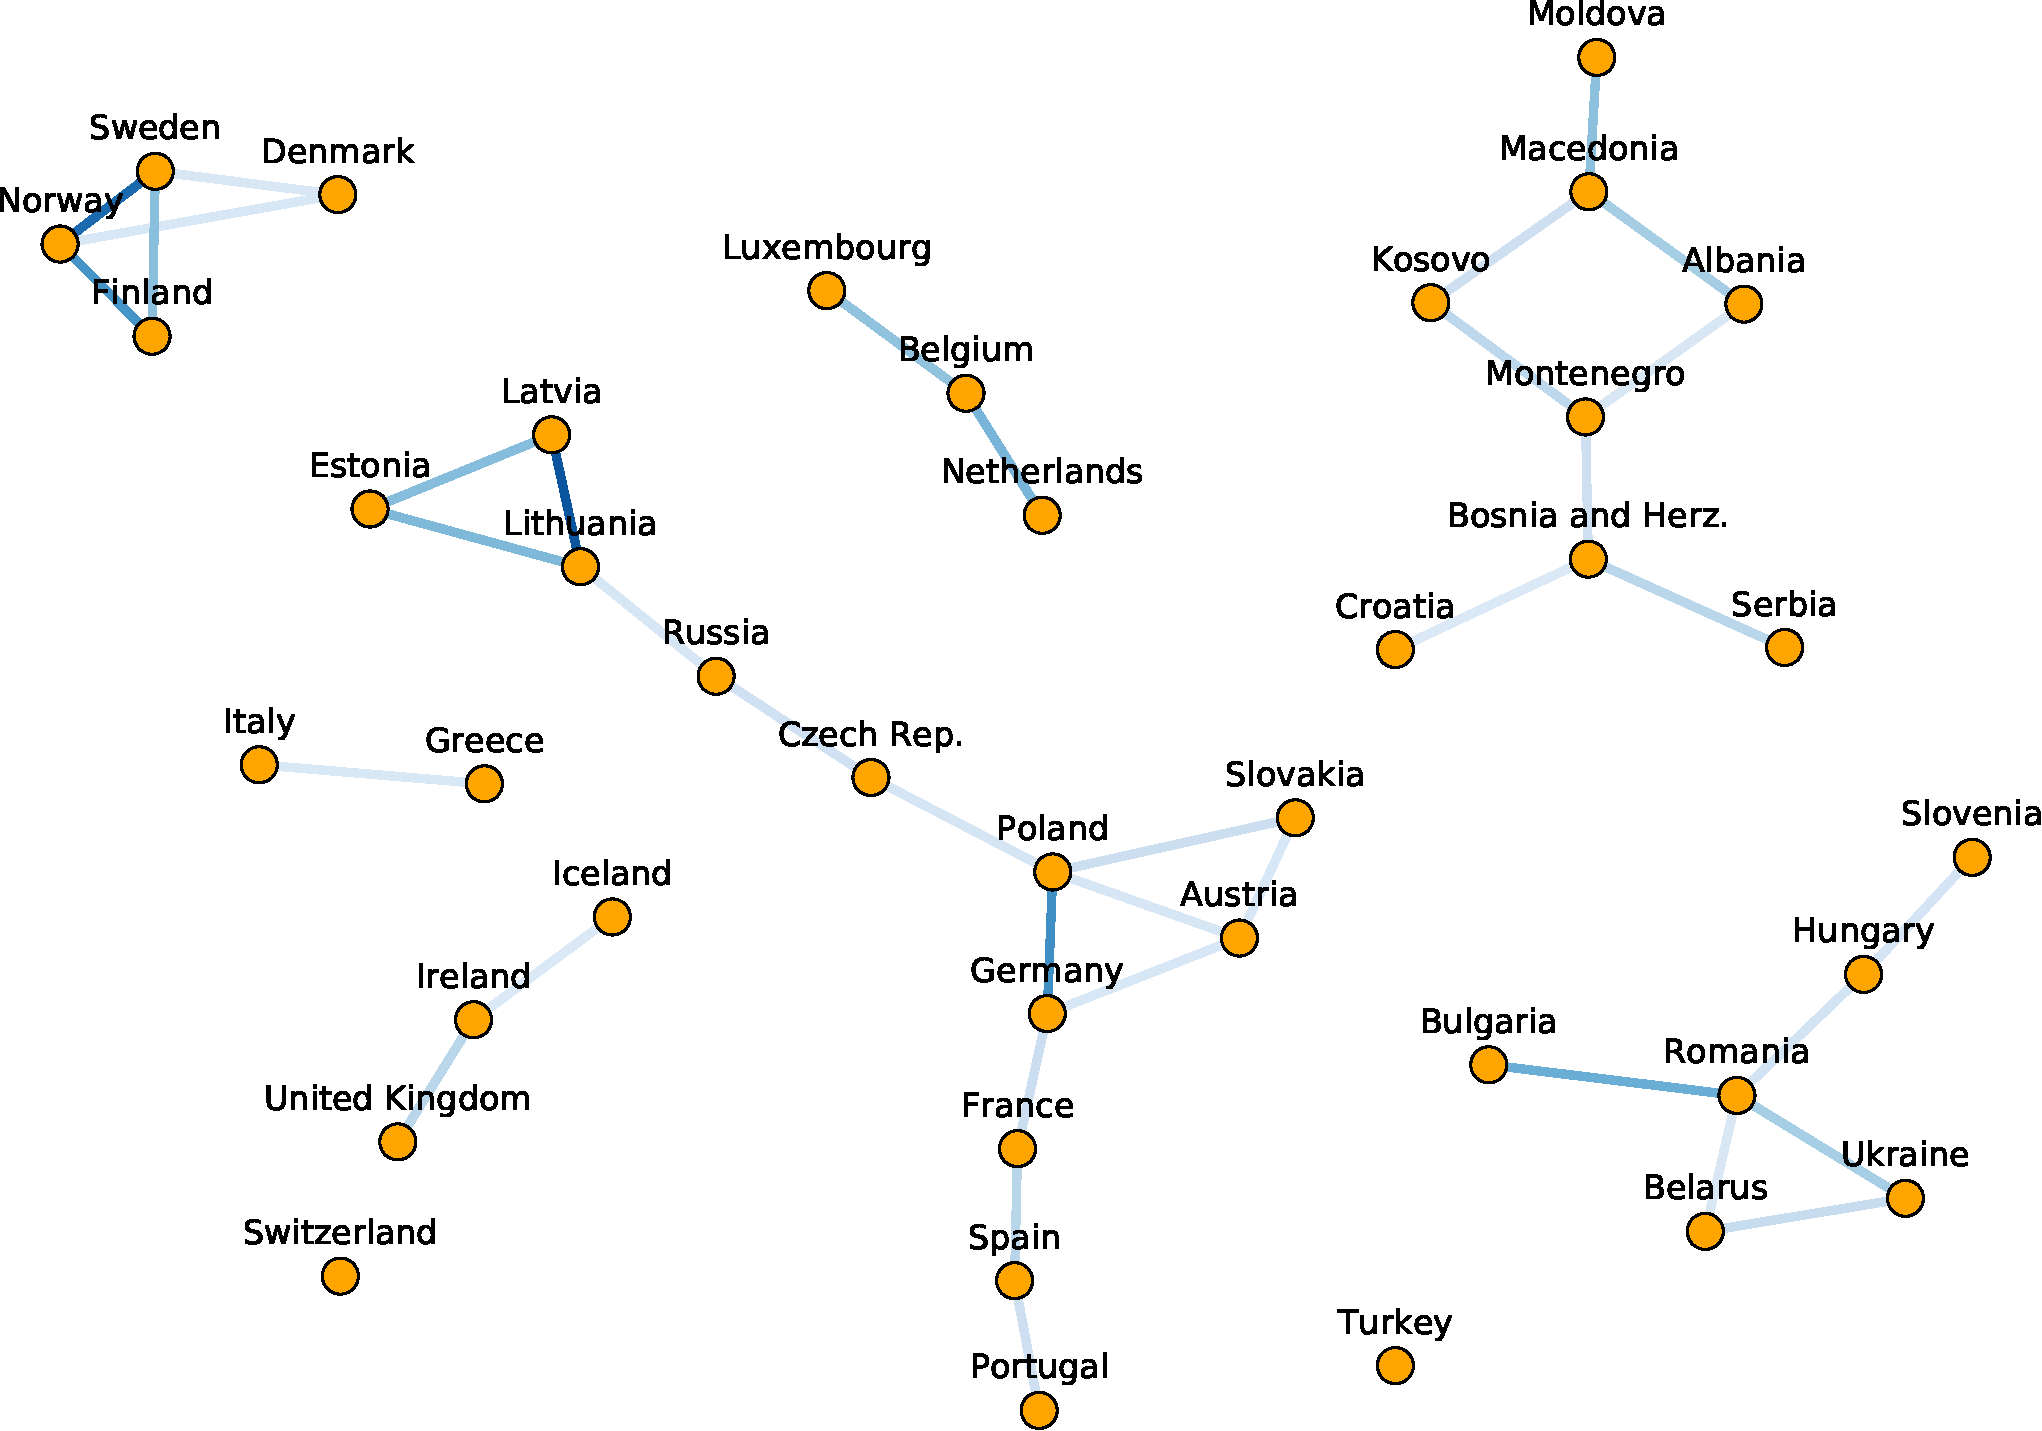
\includegraphics[width=\textwidth]{img/confusion-network}
  \caption{Confusion network of European countries. The edges between countries represent confusion of students. Dark blue edge means that the two connected countries are confused by students quite often while light blue indicates that the countries are still sometimes confused but at least less often.}
  \label{fig:confusion-network}
\end{figure}

A completely different approach on student modeling is the usage of Recurrent Neural Networks (RNNs), the family of RNN model have important advantage over models analyzed in our thesis---they do not require explicit encoding of the essential aspects of human memory and can capture more complex patterns of learning. The usage of RNNs in education, especially the Long Short Term Memory (LSTM) model, has been already explored and shows promising results~\cite{piech2015deep}. It might be interesting to analyze the RNN model in the context of the system for learning geography and also compare the performance with PFA models.
